Two parameters of the model, the \textbf{\textit{in vivo} growth rate $r$ of A20 mCherry cells} and the \textbf{cytotoxicity rate $\mu_{AC}$} in the presence of drug, were experimentally derived with an \textit{in vivo} approach, for which 20 murine models were considered. \par
\vspace{0.4cm}
To measure the instantaneous growth rate, 20 mice were inoculated with A20 murine leukemic cells. On day 16 after inoculation, blood was collected from the tail veins of four randomly chosen mice, and again on day 22 from four other mice. The proportion of A20 cells over the total was estimated using flow cytometry. Assuming a logistic growth (appropriate for cancer growth, since it takes place in a competitive environment with limited resources), we can compute the instantaneous growth rate as: 
\[ r = \frac{\ln{N(t)/N(0)}}{t} = \frac{\ln{16338/3662}}{144} = 0.01\ h^{-1} \]
Where $N(0), N(t)$ are the number of cells at times $0$ (16 days after inoculation) and $t$ (22 days, and so 144 hours, after inoculation).\\ \par
\vspace{0.4cm}
For what concerns $\mu_{AC}$, we notice that it's a crucial parameter for the model, since it represents the efficiency with whom a drug is able to kill cancer cells. Researchers were interested in computing $\mu_{AC}$, by the means of \textit{in vivo} experiments on murine model bearing the A20 cells, for the effect of two different drugs, Cytarabine (Cyt) and Ibrutinib (Ibr), in different doses. To apply the desired protocols, developed after reviewing the literature in which Cyt and Ibr had been used \textit{in vivo}, researchers divided the 20 mice in 5 different groups:\begin{enumerate}
	\item Control group, which only received PBS.
	\item Cyt Low group, which received $0.12$ mg/kg of Cyt for 5 days. This is equivalent to injecting $5.94 \cdot 10^{15}$ molecules of Cyt at each
	administration. 
	\item Cyt High group, which received $62.5$ mg/kg of Cyt for 3 days. This is equivalent to injecting $3 \cdot 10^{18}$ molecules of Cyt at each
	administration. 
	\item Ibr Low group, which received $9$ mg/kg of Ibr in days 1-5 and 8-10. This is equivalent to injecting $2.5 \cdot 10^{17}$ molecules of Ibr at 
	each administration. 
	\item Ibr High group, which received $18$ mg/kg of Ibr on days 1–5 and 8–10. This is equivalent to injecting $5 \cdot 10^{17}$ molecules of Ibr at 
	each administration. 
\end{enumerate}
To estimate $\mu_{AC}$ in groups 2 to 5, blood was collected from all mice, on the day of the initiation of the treatment and 2 days after the last treatment. At each of the two time points and in each treated mouse, the percent change in the frequency of A20 cells relative to the average
frequency in the control group was calculated. Then, for each treated group, these individual measurements were then averaged. This led to the estimation of the \textit{experimental cell growth inhibition percentage} for the 4 treated groups. \par
\begin{figure} [h]
\centering
\begin{subfigure}{0.49\textwidth}
\centering
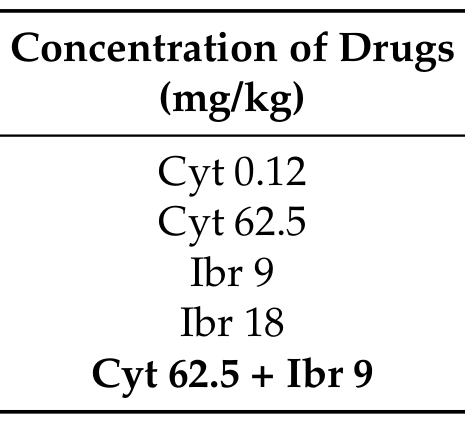
\includegraphics[scale = 0.18] {conc.png}
\end{subfigure}
\begin{subfigure}{0.49\textwidth}
\centering
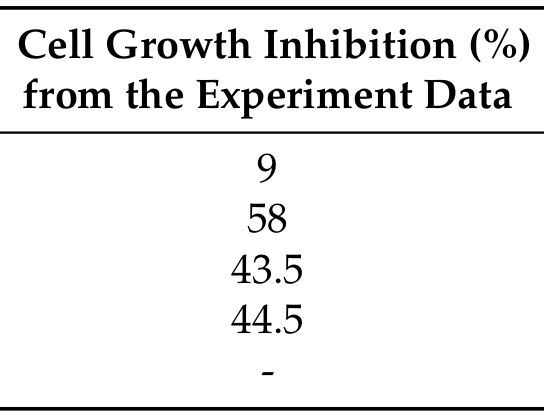
\includegraphics [scale = 0.18] {inhibition.png}
\end{subfigure}
\end{figure}
We notice that growth inhibition due to Cyt was dose dependent, whereas inhibition due to Ibr was not. At this point, a total of 12 deterministic simulations were performed, 3 for each treatment group, using $(A = 5.4 \cdot 10^{4}, E = 2500, C = 0)$ as starting point. In the context of the same treatment group, the simulations set themselves apart for the numerical choice of $\mu_{AC}$: Cyt Low was tested with $\mu_{Ac} = 0.0001$, $\mu_{Ac} = 0.001$ and $\mu_{Ac} = 0.003$. Cyt High was tested with $\mu_{Ac} = 0.005$, $\mu_{Ac} = 0.012$, $\mu_{Ac} = 0.02$. Ibr Low was tested with $\mu_{Ac} = 0.001$, $\mu_{Ac} = 0.0041$, $\mu_{Ac} = 0.005$. Ibr High with $\mu_{Ac} = 0.002$, $\mu_{Ac} = 0.0042$, $\mu_{Ac} = 0.006$. Black lines represent cancer evolution without treatment. The goal was finding, for each treatment protocol, the value for $\mu_{Ac}$, among the one proposed, that gives a \textit{simulated cell growth inhibition percentage} similar for the one obtained from the experiments. 
\begin{figure} [h]
    \centering
    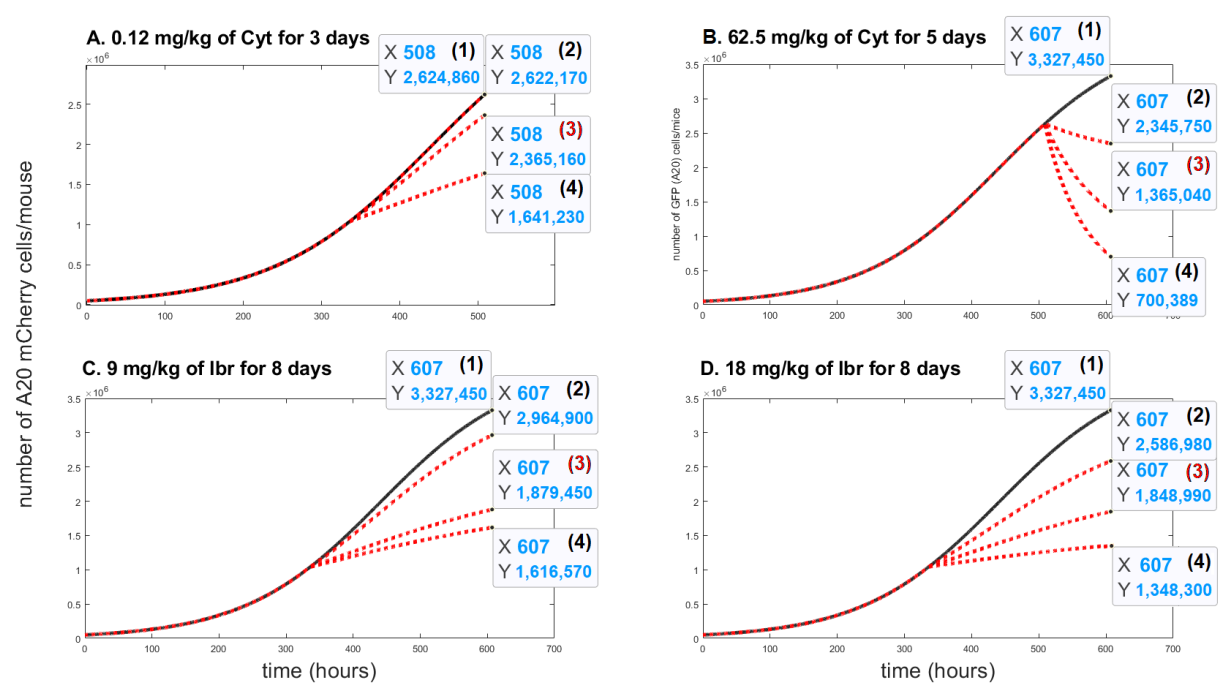
\includegraphics [scale = 0.26] {4.png}
\end{figure}
\begin{itemize}
    \item Cyt Low has a target cell growth inhibition percentage of $9 \%$. This is best reached by using $\mu_{Ac} = 0.001$, that provided $10 \%$ of growth inhibition. 
    \item Cyt High has a target cell growth inhibition percentage of $58 \%$. This is best reached by using $\mu_{Ac} = 0.012$, that provided $59 \%$ of growth inhibition. 
    \item Ibr Low has a target cell growth inhibition percentage of $43.5 \%$. This is best reached by using $\mu_{Ac} = 0.0041$, that provided $43.4 \%$ of growth inhibition. 
    \item Ibr High has a target cell growth inhibition percentage of $44.5 \%$. This is best reached by using $\mu_{Ac} = 0.0042$, that provided $44 \%$ of growth inhibition. 
\end{itemize}
\begin{figure} [h]
    \centering
    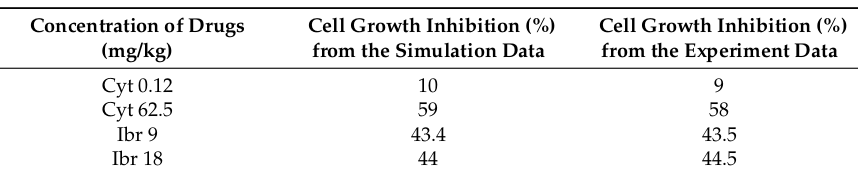
\includegraphics [scale = 0.4] {table.png}
\end{figure}

